\documentclass[11pt]{article}
\usepackage{amsmath}
\usepackage{amssymb}
\usepackage{graphicx}
\usepackage{tabularx}
\usepackage{fancyhdr}
\usepackage{lastpage}

% Page layout
\usepackage[top=1in, bottom=1in, left=1in, right=1in]{geometry}

% Header and footer
\pagestyle{fancy}
\fancyhf{}
\rfoot{Page \thepage}
\renewcommand{\headrulewidth}{0pt}

% Modified Question command with left-aligned number
\newcommand{\questiona}[2]{
    \noindent\textbf{Q#2.} #1 \hfill \textbf{[1 Mark]}
}

\newcommand{\questionb}[2]{
    \noindent\textbf{Q#2.} #1 \hfill \textbf{[2 Marks]}
}

\begin{document}

% Title section with horizontal line
\begin{center}
    \Large\textbf{GATE 2018 - Computer Science (CS)} \\
    \large\textbf{General Aptitude and Technical Questions} \\
    \rule{\textwidth}{0.5pt}
\end{center}

\vspace{0.5cm}

\section*{General Aptitude}

\questiona{“From where are they bringing their books? \_\_\_\_\_ bringing \_\_\_\_\_ books from \_\_\_\_\_.”}{1}
\begin{enumerate}
    \item[(A)] Their, they’re, there
    \item[(B)] They’re, their, there
    \item[(C)] There, their, they’re
    \item[(D)] They’re, there, there
\end{enumerate}
\vspace{0.5cm}

\questiona{“A \_\_\_\_\_\_\_ investigation can sometimes yield new facts, but typically organized ones are more successful.”}{2}
\begin{enumerate}
    \item[(A)] meandering
    \item[(B)] timely
    \item[(C)] consistent
    \item[(D)] systematic
\end{enumerate}
\vspace{0.5cm}

\questiona{The area of a square is \( d \). What is the area of the circle which has the diagonal of the square as its diameter?}{3}
\begin{enumerate}
    \item[(A)] \( \pi d \)
    \item[(B)] \( \pi d^2 \)
    \item[(C)] \( \frac{1}{4}\pi d^2 \)
    \item[(D)] \( \frac{1}{2}\pi d \)
\end{enumerate}
\vspace{0.5cm}

\questiona{What would be the smallest natural number which when divided either by 20 or by 42 or by 76 leaves a remainder of 7 in each case?}{4}
\begin{enumerate}
    \item[(A)] 3047
    \item[(B)] 6047
    \item[(C)] 7987
    \item[(D)] 63847
\end{enumerate}
\vspace{0.5cm}

\questiona{What is the missing number in the following sequence?\\
2, 12, 60, 240, 720, 1440, \_\_\_\_, 0}{5}
\begin{enumerate}
    \item[(A)] 2880
    \item[(B)] 1440
    \item[(C)] 720
    \item[(D)] 0
\end{enumerate}
\vspace{0.5cm}

\questionb{In appreciation of the social improvements completed in a town, a wealthy philanthropist decided to gift Rs 750 to each male senior citizen in the town and Rs 1000 to each female senior citizen. Altogether, there were 300 senior citizens eligible for this gift. However, only \( \frac{8}{9} \) of the eligible men and \( \frac{2}{3} \) of the eligible women claimed the gift. How much money (in Rupees) did the philanthropist give away in total?}{6}
\begin{enumerate}
    \item[(A)] 1,50,000
    \item[(B)] 2,00,000
    \item[(C)] 1,75,000
    \item[(D)] 1,51,000
\end{enumerate}
\vspace{0.5cm}

\questionb{If \( pqr \neq 0 \) and \( p - x = \frac{1}{q}, q - y = \frac{1}{r}, r - z = \frac{1}{p} \), what is the value of the product \( xyz \)?}{7}
\begin{enumerate}
    \item[(A)] -1
    \item[(B)] \( \frac{1}{pqr} \)
    \item[(C)] 1
    \item[(D)] \( pqr \)
\end{enumerate}
\vspace{0.5cm}

\questionb{In a party, 60\% of the invited guests are male and 40\% are female. If 80\% of the invited guests attended the party and if all the invited female guests attended, what would be the ratio of males to females among the attendees in the party?}{8}
\begin{enumerate}
    \item[(A)] 2:3
    \item[(B)] 1:1
    \item[(C)] 3:2
    \item[(D)] 2:1
\end{enumerate}
\vspace{0.5cm}

\questionb{In the figure below, \( \angle DEC + \angle BFC \) is equal to \_\_\_\_\_\_\_\_.}{9}
\begin{center}
    
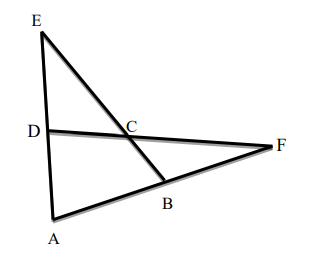
\includegraphics[width=0.5\textwidth]{figures/9}
\end{center}


\begin{enumerate}
    \item[(A)] \( \angle BCD - \angle BAD \)
    \item[(B)] \( \angle BAD + \angle BCF \)
    \item[(C)] \( \angle BAD + \angle BCD \)
    \item[(D)] \( \angle CBA + \angle ADC \)
\end{enumerate}
\vspace{0.5cm}

\questionb{A six-sided unbiased die with four green faces and two red faces is rolled seven times. Which of the following combinations is the most likely outcome of the experiment?}{10}
\begin{enumerate}
    \item[(A)] Three green faces and four red faces
    \item[(B)] Four green faces and three red faces
    \item[(C)] Five green faces and two red faces
    \item[(D)] Six green faces and one red face
\end{enumerate}
\vspace{0.5cm}

\section*{Technical Section}

\questiona{Which one of the following is a closed form expression for the generating function of the sequence \( \{a_n\} \), where \( a_n = 2n + 3 \) for all \( n = 0, 1, 2, \dots \)?}{1}
\begin{enumerate}
    \item[(A)] \( \frac{2}{3(1 - x)} \)
    \item[(B)] \( \frac{2x}{3(1 - x)} \)
    \item[(C)] \( \frac{2x^2}{(1 - x)^2} \)
    \item[(D)] \( \frac{2x}{(1 - x)^2} \)
\end{enumerate}
\vspace{0.5cm}

\questiona{Consider the following C program:
\begin{center}
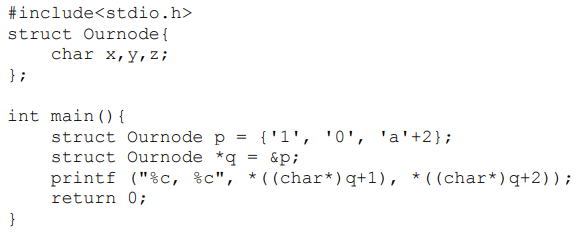
\includegraphics[width=0.6\textwidth]{figures/2.png}
\end{center}
The output of this program is:}{2}
\begin{enumerate}
    \item[(A)] 0, c
    \item[(B)] 0, a+2
    \item[(C)] '0', 'a+2'
    \item[(D)] '0', 'c'
\end{enumerate}
\vspace{0.5cm}

\questiona{A queue is implemented using a non-circular singly linked list. The queue has a head pointer and a tail pointer. Let \( n \) denote the number of nodes in the queue. Let enqueue be implemented by inserting a new node at the head, and dequeue be implemented by deletion of a node from the tail.
\begin{center}
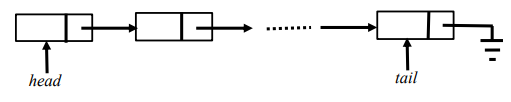
\includegraphics[width=0.5\textwidth]{figures/3.png}
\end{center}
Which one of the following is the time complexity of the most time-efficient implementation of enqueue and dequeue, respectively, for this data structure?}{3}
\begin{enumerate}
    \item[(A)] \( \Theta(1), \Theta(1) \)
    \item[(B)] \( \Theta(1), \Theta(n) \)
    \item[(C)] \( \Theta(n), \Theta(1) \)
    \item[(D)] \( \Theta(n), \Theta(n) \)
\end{enumerate}
\vspace{0.5cm}

\questiona{Let \( \oplus \) and \( \odot \) denote the Exclusive OR and Exclusive NOR operations, respectively. Which one of the following is NOT CORRECT?}{4}
\begin{enumerate}
    \item[(A)] \( P \oplus \overline{Q} = P \odot Q \)
    \item[(B)] \( \overline{P} \oplus Q = P \odot Q \)
    \item[(C)] \( \overline{P} \oplus \overline{Q} = P \oplus Q \)
    \item[(D)] \( (P \oplus \overline{Q}) \oplus Q = (P \odot \overline{Q}) \odot \overline{Q} \)
\end{enumerate}
\vspace{0.5cm}

\questiona{Consider the following processor design characteristics.\\
I. Register-to-register arithmetic operations only\\
II. Fixed-length instruction format\\
III. Hardwired control unit\\
Which of the characteristics above are used in the design of a RISC processor?}{5}
\begin{enumerate}
    \item[(A)] I and II only
    \item[(B)] II and III only
    \item[(C)] I and III only
    \item[(D)] I, II and III
\end{enumerate}
\vspace{0.5cm}

\questiona{Let \( N \) be an NFA with \( n \) states. Let \( k \) be the number of states of a minimal DFA which is equivalent to \( N \). Which one of the following is necessarily true?}{6}
\begin{enumerate}
    \item[(A)] \( k \geq 2^n \)
    \item[(B)] \( k \geq n \)
    \item[(C)] \( k \leq n^2 \)
    \item[(D)] \( k \leq 2^n \)
\end{enumerate}
\vspace{0.5cm}

\questiona{The set of all recursively enumerable languages is}{7}
\begin{enumerate}
    \item[(A)] closed under complementation.
    \item[(B)] closed under intersection.
    \item[(C)] a subset of the set of all recursive languages.
    \item[(D)] an uncountable set.
\end{enumerate}
\vspace{0.5cm}

\questiona{Which one of the following statements is FALSE?}{8}
\begin{enumerate}
    \item[(A)] Context-free grammar can be used to specify both lexical and syntax rules.
    \item[(B)] Type checking is done before parsing.
    \item[(C)] High-level language programs can be translated to different Intermediate Representations.
    \item[(D)] Arguments to a function can be passed using the program stack.
\end{enumerate}
\vspace{0.5cm}

\questiona{The following are some events that occur after a device controller issues an interrupt while process \( L \) is under execution.\\
(P) The processor pushes the process status of \( L \) onto the control stack.\\
(Q) The processor finishes the execution of the current instruction.\\
(R) The processor executes the interrupt service routine.\\
(S) The processor pops the process status of \( L \) from the control stack.\\
(T) The processor loads the new PC value based on the interrupt.\\
Which one of the following is the correct order in which the events above occur?}{9}
\begin{enumerate}
    \item[(A)] QPTRS
    \item[(B)] PTRSQ
    \item[(C)] TRPQS
    \item[(D)] QTPRS
\end{enumerate}
\vspace{0.5cm}

\questiona{Consider a process executing on an operating system that uses demand paging. The average time for a memory access in the system is \( M \) units if the corresponding memory page is available in memory, and \( D \) units if the memory access causes a page fault. It has been experimentally measured that the average time taken for a memory access in the process is \( X \) units. Which one of the following is the correct expression for the page fault rate experienced by the process?}{10}
\begin{enumerate}
    \item[(A)] \( \frac{D - M}{X - M} \)
    \item[(B)] \( \frac{X - M}{D - M} \)
    \item[(C)] \( \frac{D - X}{D - M} \)
    \item[(D)] \( \frac{X - M}{D - X} \)
\end{enumerate}
\vspace{0.5cm}

\questiona{In an Entity-Relationship (ER) model, suppose \( R \) is a many-to-one relationship from entity set \( E_1 \) to entity set \( E_2 \). Assume that \( E_1 \) and \( E_2 \) participate totally in \( R \) and that the cardinality of \( E_1 \) is greater than the cardinality of \( E_2 \). Which one of the following is true about \( R \)?}{11}
\begin{enumerate}
    \item[(A)] Every entity in \( E_1 \) is associated with exactly one entity in \( E_2 \).
    \item[(B)] Some entity in \( E_1 \) is associated with more than one entity in \( E_2 \).
    \item[(C)] Every entity in \( E_2 \) is associated with exactly one entity in \( E_1 \).
    \item[(D)] Every entity in \( E_2 \) is associated with at most one entity in \( E_1 \).
\end{enumerate}
\vspace{0.5cm}

\questiona{Consider the following two tables and four queries in SQL.\\
\texttt{Book(isbn, bname), Stock(isbn, copies)}\\
Query 1: \texttt{SELECT B.isbn, S.copies FROM Book B INNER JOIN Stock S ON B.isbn = S.isbn;}\\
Query 2: \texttt{SELECT B.isbn, S.copies FROM Book B LEFT OUTER JOIN Stock S ON B.isbn = S.isbn;}\\
Query 3: \texttt{SELECT B.isbn, S.copies FROM Book B RIGHT OUTER JOIN Stock S ON B.isbn = S.isbn;}\\
Query 4: \texttt{SELECT B.isbn, S.copies FROM Book B FULL OUTER JOIN Stock S ON B.isbn = S.isbn;}\\
Which one of the queries above is certain to have an output that is a superset of the outputs of the other three queries?}{12}
\begin{enumerate}
    \item[(A)] Query 1
    \item[(B)] Query 2
    \item[(C)] Query 3
    \item[(D)] Query 4
\end{enumerate}
\vspace{0.5cm}

\questiona{Match the following:\\
\begin{tabular}{ll}
P. UDP Header’s Port Number & I. 48 \\
Q. Ethernet MAC Address & II. 8 \\
R. IPv6 Next Header & III. 32 \\
S. TCP Header’s Sequence Number & IV. 16 \\
\end{tabular}}{13}
\begin{enumerate}
    \item[(A)] P-III, Q-IV, R-II, S-I
    \item[(B)] P-II, Q-I, R-IV, S-III
    \item[(C)] P-IV, Q-I, R-II, S-III
    \item[(D)] P-IV, Q-I, R-III, S-II
\end{enumerate}
\vspace{0.5cm}

\questiona{Consider the following statements regarding the slow start phase of the TCP congestion control algorithm. Let cwnd denote the TCP congestion window and MSS the Maximum Segment Size.\\
(i) The cwnd increases by 2 MSS on every successful acknowledgment.\\
(ii) The cwnd approximately doubles on every successful acknowledgement.\\
(iii) The cwnd increases by 1 MSS every round trip time.\\
(iv) The cwnd approximately doubles every round trip time.\\
Which one of the following is correct?}{14}
\begin{enumerate}
    \item[(A)] Only (ii) and (iii) are true
    \item[(B)] Only (i) and (iii) are true
    \item[(C)] Only (iv) is true
    \item[(D)] Only (i) and (iv) are true
\end{enumerate}
\vspace{0.5cm}

\questiona{Two people, P and Q, roll two identical dice. The person with the lower number wins. In case of a tie, they roll again until there is no tie. Define a trial as one roll by both. Assume fair dice and independence. The probability (rounded to 3 decimal places) that one of them wins on the third trial is \_\_\_\_.}{15}
\vspace{0.5cm}

\questiona{The value of \( \int_0^{\pi/4} x \cos(x^2) dx \), correct to three decimal places (assuming \( \pi = 3.14 \)), is \_\_\_\_.}{16}
\vspace{0.5cm}

\questiona{Consider a matrix \( A = uv^T \) where \( u = \begin{bmatrix} 1 \\\\ 1 \end{bmatrix}, v = \begin{bmatrix} 2 \\\\ 1 \end{bmatrix} \). The largest eigenvalue of \( A \) is \_\_\_\_.}{17}
\vspace{0.5cm}

\questiona{The chromatic number of the following graph is \_\_\_\_.}{18}
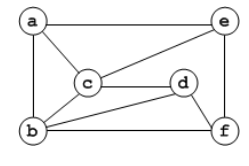
\includegraphics[width=0.5\textwidth]{figures/18}
\vspace{0.5cm}

\questiona{Let \( G \) be a finite group on 84 elements. The size of the largest possible proper subgroup of \( G \) is \_\_\_\_.}{19}
\vspace{0.5cm}

\questiona{The postorder traversal of a binary tree is 8,9,6,7,4,5,2,3,1. The inorder traversal of the same tree is 8,6,9,4,7,2,5,1,3. The height of the binary tree is \_\_\_\_.}{20}
\vspace{0.5cm}

\questiona{Consider the following C program:\\
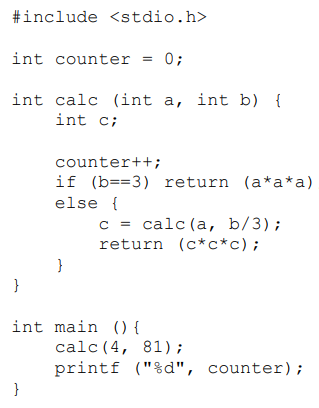
\includegraphics[width=0.5\textwidth]{figures/21}\\
The output of this program is \_\_\_\_.}{21}
\vspace{0.5cm}

\questiona{Consider the sequential circuit shown in the figure below, where both flip-flops are positive edge-triggered D flip-flops. The number of states in the state transition diagram of this circuit that have a transition back to the same state on some value of “in” is \_\_\_\_.}{22}
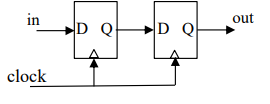
\includegraphics[width=0.5\textwidth]{figures/22}
\vspace{0.5cm}

\questiona{A 32-bit wide main memory unit with a capacity of 1 GB is built using 256M × 4-bit DRAM chips. The number of rows of memory cells in the DRAM chip is \( 2^{14} \). The time taken to perform one refresh operation is 50 nanoseconds. The refresh period is 2 milliseconds. The percentage (rounded to the closest integer) of the time available for performing memory read/write operations in the main memory unit is \_\_\_\_.}{23}
\vspace{0.5cm}

\questiona{Consider a system with 3 processes that share 4 instances of the same resource type. Each process can request a maximum of \( K \) instances. Resource instances can be requested and released only one at a time. The largest value of \( K \) that will always avoid deadlock is \_\_\_\_.}{24}
\vspace{0.5cm}

\questiona{Consider a long-lived TCP session with an end-to-end bandwidth of 1 Gbps (= \(10^9\) bits-per-second). The session starts with a sequence number of 1234. The minimum time (in seconds, rounded to the closest integer) before this sequence number can be used again is \_\_\_\_.}{25}
\vspace{0.5cm}

\questionb{Consider a matrix \( P \) whose only eigenvectors are the multiples of \( \begin{bmatrix} 1 \\\\ 4 \end{bmatrix} \).\\
Which one of the following options is correct?\\
(I) \( P \) does not have an inverse\\
(II) \( P \) has a repeated eigenvalue\\
(III) \( P \) cannot be diagonalized}{26}
\begin{enumerate}
    \item[(A)] Only I and III are necessarily true
    \item[(B)] Only II is necessarily true
    \item[(C)] Only I and II are necessarily true
    \item[(D)] Only II and III are necessarily true
\end{enumerate}
\vspace{0.5cm}

\questionb{Let \( N \) be the set of natural numbers. Consider the following sets:\\
P: Set of Rational numbers (positive and negative)\\
Q: Set of functions from \( \{0,1\} \) to \( N \)\\
R: Set of functions from \( N \) to \( \{0,1\} \)\\
S: Set of finite subsets of \( N \)\\
Which of the sets above are countable?}{27}
\begin{enumerate}
    \item[(A)] Q and S only
    \item[(B)] P and S only
    \item[(C)] P and R only
    \item[(D)] P, Q and S only
\end{enumerate}
\vspace{0.5cm}

\questionb{Consider the first-order logic sentence\\
\( \phi \equiv \exists s \exists t \exists u \forall v \forall w \forall x \forall y \; \psi(s,t,u,v,w,x,y) \)\\
where \( \psi \) is quantifier-free and contains only predicate symbols and possibly equality, but no function symbols. Suppose \( \phi \) has a model with universe size 7. Which one of the following statements is necessarily true?}{28}
\begin{enumerate}
    \item[(A)] There exists at least one model of \( \phi \) with universe of size \( \leq 3 \)
    \item[(B)] There exists no model of \( \phi \) with universe of size \( \leq 3 \)
    \item[(C)] There exists no model of \( \phi \) with universe of size greater than 7
    \item[(D)] Every model of \( \phi \) has a universe of size equal to 7
\end{enumerate}
\vspace{0.5cm}

\questionb{Consider the following C program:\\
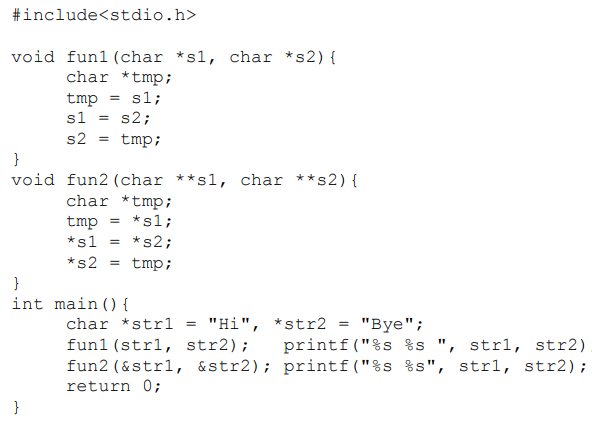
\includegraphics[width=0.5\textwidth]{figures/29}\\
The output of the program above is}{29}
\begin{enumerate}
    \item[(A)] Hi Bye Bye Hi
    \item[(B)] Hi Bye Hi Bye
    \item[(C)] Bye Hi Hi Bye
    \item[(D)] Bye Hi Bye Hi
\end{enumerate}
\vspace{0.5cm}

\questionb{Let \( G \) be a simple undirected graph. Let \( T_D \) be a depth-first search tree of \( G \). Let \( T_B \) be a breadth-first search tree of \( G \).\\
Consider the following statements:\\
(I) No edge of \( G \) is a cross edge with respect to \( T_D \).\\
(II) For every edge \( (u,v) \in G \), if \( u \) is at depth \( i \) and \( v \) is at depth \( j \) in \( T_B \), then \( |i-j| = 1 \).\\
Which of the statements above must necessarily be true?}{30}
\begin{enumerate}
    \item[(A)] I only
    \item[(B)] II only
    \item[(C)] Both I and II
    \item[(D)] Neither I nor II
\end{enumerate}
\vspace{0.5cm}

\questionb{Assume multiplying a matrix \( G_1 \) of dimension \( p \times q \) with \( G_2 \) of dimension \( q \times r \) requires \( pqr \) scalar multiplications. In a multiplication chain \( F_1F_2F_3F_4F_5 \), matrix dimensions are \( F_1(2 \times 25), F_2(25 \times 3), F_3(3 \times 16), F_4(16 \times 1), F_5(1 \times 1000) \). In the optimal parenthesization, which are the explicitly computed pairs?}{31}
\begin{enumerate}
    \item[(A)] \( F_1F_2 \) and \( F_3F_4 \) only
    \item[(B)] \( F_2F_3 \) only
    \item[(C)] \( F_3F_4 \) only
    \item[(D)] \( F_1F_2 \) and \( F_4F_5 \) only
\end{enumerate}
\vspace{0.5cm}

\questionb{Consider the following C code. Assume unsigned long int type length is 64 bits.\\
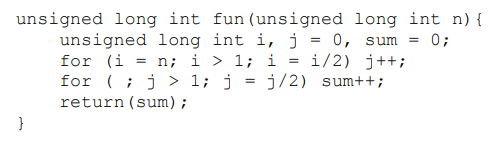
\includegraphics[width=0.5\textwidth]{figures/32}\\
The value returned when we call \texttt{fun(240)} is}{32}
\begin{enumerate}
    \item[(A)] 4
    \item[(B)] 5
    \item[(C)] 6
    \item[(D)] 40
\end{enumerate}
\vspace{0.5cm}

\questionb{Consider the unsigned 8-bit fixed-point binary number representation:\\
\[
b_7\ b_6\ b_5\ b_4\ b_3\ .\ b_2\ b_1\ b_0
\]
where the binary point is between \( b_3 \) and \( b_2 \). Assume \( b_7 \) is the most significant bit.\\
Some of the decimal numbers listed below cannot be represented exactly in the above representation:\\
(i) 31.500 \quad (ii) 0.875 \quad (iii) 12.100 \quad (iv) 3.001\\
Which one of the following statements is true?}{33}
\begin{enumerate}
    \item[(A)] None of (i), (ii), (iii), (iv) can be exactly represented
    \item[(B)] Only (ii) cannot be exactly represented
    \item[(C)] Only (iii) and (iv) cannot be exactly represented
    \item[(D)] Only (i) and (ii) cannot be exactly represented
\end{enumerate}
\vspace{0.5cm}

\questionb{The size of the physical address space of a processor is \( 2^P \) bytes. The word length is \( 2^W \) bytes. The cache memory capacity is \( 2^N \) bytes. Each cache block is \( 2^M \) words. For a \( K \)-way set-associative cache, the tag field length (in bits) is:}{34}
\begin{enumerate}
    \item[(A)] \( P - N - \log_2 K \)
    \item[(B)] \( P - N + \log_2 K \)
    \item[(C)] \( P - N - M - W - \log_2 K \)
    \item[(D)] \( P - N - M - W + \log_2 K \)
\end{enumerate}
\vspace{0.5cm}

\questionb{Consider the following languages:\\
I. \( \{ a^m b^n c^p d^q \mid m + p = n + q,\ m,n,p,q \geq 0 \} \)\\
II. \( \{ a^m b^n c^p d^q \mid m = n,\ p = q,\ m,n,p,q \geq 0 \} \)\\
III. \( \{ a^m b^n c^p d^q \mid m = n = p,\ p \neq q,\ m,n,p,q \geq 0 \} \)\\
IV. \( \{ a^m b^n c^p d^q \mid mn = p + q,\ m,n,p,q \geq 0 \} \)\\
Which of the languages above are context-free?}{35}
\begin{enumerate}
    \item[(A)] I and IV only
    \item[(B)] I and II only
    \item[(C)] II and III only
    \item[(D)] II and IV only
\end{enumerate}
\vspace{0.5cm}

\questionb{Consider the following problems where \( L(G) \) denotes the language generated by grammar \( G \), and \( L(M) \) denotes the language accepted by machine \( M \):\\
(I) For unrestricted grammar \( G \) and string \( w \), whether \( w \in L(G) \)\\
(II) Given a Turing machine \( M \), whether \( L(M) \) is regular\\
(III) Given grammars \( G_1 \) and \( G_2 \), whether \( L(G_1) = L(G_2) \)\\
(IV) Given an NFA \( N \), whether there is a deterministic PDA \( P \) such that \( N \) and \( P \) accept the same language\\
Which one of the following statements is correct?}{36}
\begin{enumerate}
    \item[(A)] Only I and II are undecidable
    \item[(B)] Only III is undecidable
    \item[(C)] Only II and IV are undecidable
    \item[(D)] Only I, II and III are undecidable
\end{enumerate}
\vspace{0.5cm}

\questionb{A lexical analyzer uses the following patterns to recognize three tokens over the alphabet \{a, b, c\}:\\
\[
T1: a? (b|c)^* a \qquad
T2: b? (a|c)^* b \qquad
T3: c? (b|a)^* c
\]
The analyzer matches the longest possible prefix.\\
If the string \texttt{bbaacabc} is processed, which of the following is the sequence of tokens output?}{37}
\begin{enumerate}
    \item[(A)] T1 T2 T3
    \item[(B)] T1 T1 T3
    \item[(C)] T2 T1 T3
    \item[(D)] T3 T3
\end{enumerate}
\vspace{0.5cm}

\questionb{Consider the following parse tree for the expression \texttt{a \# b \$ c \$ d \# e \# f} involving two binary operators \$ and \#.
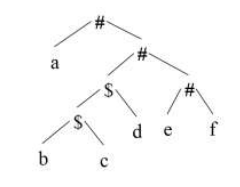
\includegraphics[width=0.5\textwidth]{figures/38}\\
Which one of the following is correct for the parse tree?}{38}
\begin{enumerate}
    \item[(A)] \$ has higher precedence and is left associative; \# is right associative
    \item[(B)] \# has higher precedence and is left associative; \$ is right associative
    \item[(C)] \$ has higher precedence and is left associative; \# is left associative
    \item[(D)] \# has higher precedence and is right associative; \$ is left associative
\end{enumerate}
\vspace{0.5cm}

\questionb{In a system, there are three types of resources: E, F, and G. Four processes \( P_0 \) to \( P_3 \) execute concurrently. Maximum resource requirements and current allocations are given.\\
Available: E=3, F=3\\
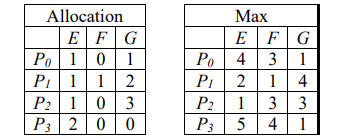
\includegraphics[width=0.5\textwidth]{figures/39}\\
From the perspective of deadlock avoidance, which of the following is true?}{39}
\begin{enumerate}
    \item[(A)] The system is in a safe state
    \item[(B)] Not in safe state, but would be if one more E were available
    \item[(C)] Not in safe state, but would be if one more F were available
    \item[(D)] Not in safe state, but would be if one more G were available
\end{enumerate}
\vspace{0.5cm}

\questionb{Consider the producer-consumer synchronization problem. The buffer size is \( N \). Semaphores: empty = 0, full = N, mutex = 1.\\
Code with placeholders P, Q, R, and S is given:\\
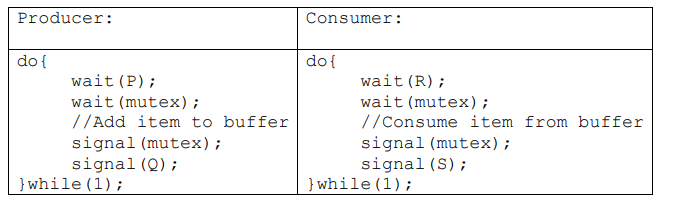
\includegraphics[width=0.5\textwidth]{figures/40}\\
Which one of the following assignments to P, Q, R, and S is correct?}{40}
\begin{enumerate}
    \item[(A)] P: full, Q: full, R: empty, S: empty
    \item[(B)] P: empty, Q: empty, R: full, S: full
    \item[(C)] P: full, Q: empty, R: empty, S: full
    \item[(D)] P: empty, Q: full, R: full, S: empty
\end{enumerate}
\vspace{0.5cm}

\questionb{Consider relations r(A, B) and s(B, C), where s.B is a primary key and r.B is a foreign key referencing s.B. Let LOJ denote the natural left outer join.\\
Which of the following queries is NOT equivalent to: \( r \bowtie (\sigma_{B<5}(s)) \)?}{41}
\begin{enumerate}
    \item[(A)] \( \sigma_{B<5}(r \bowtie s) \)
    \item[(B)] \( \sigma_{B<5}(r\ \text{LOJ}\ s) \)
    \item[(C)] \( r\ \text{LOJ}\ (\sigma_{B<5}(s)) \)
    \item[(D)] \( \sigma_{B<5}(r)\ \text{LOJ}\ s \)
\end{enumerate}
\vspace{0.5cm}

\questionb{Four relational schemas are given. Identify which one is in 3NF but not in BCNF.\\
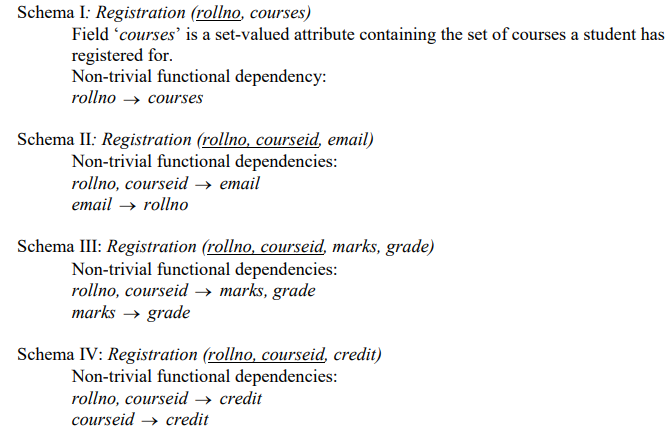
\includegraphics[width=0.5\textwidth]{figures/42}}{42}
\begin{enumerate}
    \item[(A)] Schema I
    \item[(B)] Schema II
    \item[(C)] Schema III
    \item[(D)] Schema IV
\end{enumerate}
\vspace{0.5cm}

\questionb{Let \( G \) be a graph with \( 100! \) vertices, each labeled with a distinct permutation of numbers \( 1, 2, ..., 100 \). There is an edge between vertices \( u \) and \( v \) if the label of \( u \) can be obtained by swapping two adjacent numbers in the label of \( v \). Let \( y \) denote the degree of a vertex in \( G \), and \( z \) the number of connected components in \( G \). Then, \( y + 10z = \_\_\_\_. \)}{43}
\vspace{0.5cm}

\questionb{Consider Guwahati (G) and Delhi (D) whose temperatures can be classified as high (H), medium (M), and low (L). Conditional probabilities \( P(HD|HG) = 0.40, P(MD|HG) = 0.48, P(LD|HG) = 0.12 \), etc., are given. If \( P(HG) = 0.2 \), \( P(MG) = 0.5 \), and \( P(LG) = 0.3 \), then the probability that Guwahati has high temperature given that Delhi has high temperature is \_\_\_\_.}{44}
\vspace{0.5cm}

\questionb{Consider the following pseudo-code:\\
\texttt{Count(x, y)\{\\
\hspace{0.5cm}if (y != 1) \{\\
\hspace{1cm}if (x != 1) \{ print("*"); Count(x/2, y); \}\\
\hspace{1cm}else \{ y = y - 1; Count(1024, y); \}\\
\hspace{0.5cm} \} \}}\\
The number of times the print statement executes for \texttt{Count(1024, 1024)} is \_\_\_\_.}{45}
\vspace{0.5cm}

\questionb{The number of possible min-heaps containing each value from \{1, 2, 3, 4, 5, 6, 7\} exactly once is \_\_\_\_.}{46}
\vspace{0.5cm}

\questionb{Consider the following undirected graph \( G \):\\
\begin{center}
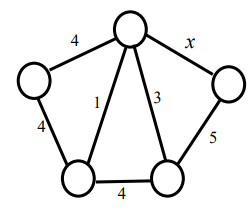
\includegraphics[width=0.5\textwidth]{figures/47}
\end{center}
Choose a value for \( x \) that maximizes the number of minimum weight spanning trees (MWSTs) of \( G \). The number of MWSTs for this value of \( x \) is \_\_\_\_.}{47}
\vspace{0.5cm}

\questionb{Consider the weights and values of items listed below. There is only one unit of each item.\\
\begin{tabular}{|c|c|c|}
\hline
Item & Weight (Kg) & Value (Rs) \\\hline
1 & 10 & 60 \\\hline
2 & 7  & 28 \\\hline
3 & 4  & 20 \\\hline
4 & 2  & 24 \\\hline
\end{tabular}\\
We can carry at most 11 Kg. The difference \( V_{opt} - V_{greedy} \) is \_\_\_\_.}{48}
\vspace{0.5cm}

\questionb{Consider the minterm list form of Boolean function \( F \):\\
\[
F(P, Q, R, S) = \sum m(0, 2, 5, 7, 9, 11) + d(3, 8, 10, 12, 14)
\]\\
The number of essential prime implicants of \( F \) is \_\_\_\_.}{49}
\vspace{0.5cm}

\questionb{A RISC processor has the following instruction pipeline stages: IF, ID, OF, PO, WB. IF, ID, OF, WB take 1 clock cycle each. PO takes 3 cycles for 40 instructions, 2 cycles for 35 instructions, and 1 cycle for 25 instructions. The number of clock cycles required to complete 100 instructions is \_\_\_\_.}{50}
\vspace{0.5cm}

\questionb{A processor has 16 integer and 64 floating point registers. It uses 2-byte instruction format. There are 4 instruction types. Type-4 uses 1 floating point register operand. The maximum number of Type-4 instructions is \_\_\_\_.}{51}
\vspace{0.5cm}

\questionb{Given a language \( L \), define \( L_0 = \{\epsilon\}, L_i = L_{i-1} \cdot L \). The order of a language is the smallest \( k \) such that \( L_k = L_{k+1} \).\\
For the following automaton:
\begin{center}
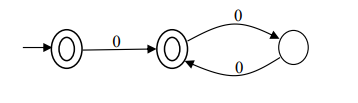
\includegraphics[width=0.5\textwidth]{figures/52}
\end{center}
The order of the language is \_\_\_\_.}{52}
\vspace{0.5cm}

\questionb{Consider a storage disk with 4 platters, 200 cylinders, 256 sectors per track. Disk requests: [120,72,2], [180,134,1], [60,20,0], [212,86,3], [56,116,2], [118,16,1]. Head is at [100, 80], moving towards higher cylinders. Power to move 100 cylinders = 20 mW, to reverse = 15 mW. Total power consumption using SSTF is \_\_\_\_ mW.}{53}
\vspace{0.5cm}

\questionb{An IP packet of 4500 bytes includes 20-byte IP header and 40-byte TCP header. The MTU is 600 bytes. IP headers of outgoing fragments are 20 bytes. The fragmentation offset of the third fragment is \_\_\_\_.}{54}
\vspace{0.5cm}

\questionb{Multiple nodes share a broadcast medium. They use a carrier-sense based protocol. P starts transmitting at time \( t = 0 \). Q also has a packet at \( t = 0 \) and begins carrier sensing. If the transmission speed is 10 meters per unit time and each transmission lasts 20 time units, the maximum distance \( d \) (rounded to the nearest integer) that avoids collision is \_\_\_\_.}{55}
\vspace{0.5cm}




\vspace{5cm}
\begin{center}
\textbf{END OF THE QUESTION PAPER} \\
\rule{\textwidth}{0.5pt}
\end{center}

\end{document}
